   
% @author Hannes Ahrens
% @date   M�rz 2009
% 
%%%%%%%%%%%%%%%%%%%%%%%%%%%%%%%%%%%%%%%%%%%%

%%%%%%%%%%%%%%%%%%%%%%%%%%%%%%%%%%%%%%%%%%%%%%%%%%
%------------- TITEL ---------------------------
%%%%%%%%%%%%%%%%%%%%%%%%%%%%%%%%%%%%%%%%%%%%%%%%%%

      
\title{Renew (File-)Navigator}
\titlerunning{Renew (File-)Navigator}

\author{Hannes Ahrens}

\institute{Department  Informatik, TGI, Universit\"at Hamburg\\
   http://www.informatik.uni-hamburg.de/TGI/\\
   4ahrens@informatik.uni-hamburg.de
 }
      

%%%%%%%%%%%%%%%%%%%%%%%%%%%%%%%%%%%%%%%%%%%%%%%%%%%
%------------- DOCUMENT -------------------------
%%%%%%%%%%%%%%%%%%%%%%%%%%%%%%%%%%%%%%%%%%%%%%%%%%%

{
\renewcommand{\textfraction}{0}

\maketitle

\begin{figure}[htp]%
\centering%
  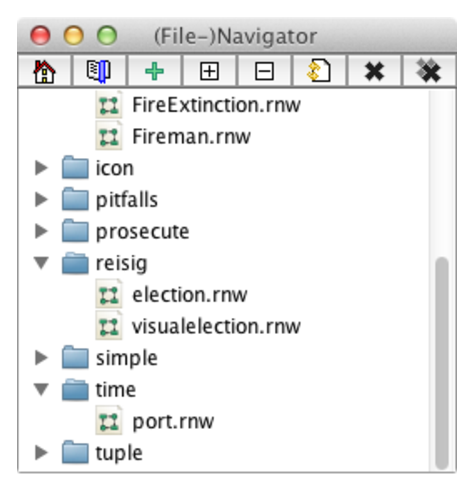
\includegraphics[height=0.6\textheight]{images/Navigator}%
  %\caption{Renew (File-)Navigator}%
  \label{fig:Navigator}%
\end{figure}

%\input{toc}
\tableofcontents

 \begin{abstract}
 Diese Projektarbeit widmet sich dem Erstellen unterschiedlicher Navigator-Plugins f"ur Renew.
 Dabei wird vorallem auf das entwickelte (File-)Navigator-Plugin eingegangen, aber es werden auch Alternativen und m"ogliche Erweiterungen aufgegriffen.
 
 	Das erstellte (File-)Navigator-Plugin erg"anzt Renew bereits um eine einfache M"oglichkeit auf Dateien zuzugreifen.
 	Es l"asst Ordner und in ihnen enthaltene Dateien darstellen, Verzeichnis"ubergreifend ausw"ahlen und "offnen. Es bietet grundlegende Funktionen zur Betrachung, sowie zum Hinzuf"ugen, Aktualisieren und Entfernen von Verzeichnissen und Dateien. Von Renew zum "Offnen nicht zugelassene Dateien werden dabei herausgefiltert.
 	Dieses Plugin mindert damit das bislang oftmals sehr umst"andliche Navigieren durch Verzeichnispfade.
 \end{abstract}


 \section{Einleitung}
 Nachdem ich das AOSE-Projekt nun zum zweiten Mal besucht habe, dr"angte sich mir der Gedanke f"ur Renew einen Datei-Navigator zu entwickeln geradezu auf.
 Nach meiner Erfahrung und vernommenen "Au{\ss}erungen verschiedener Komilitonen, ist es bislang sehr m"uhsam gewesen in Renew viele verschiedene Dateien aus verschiedenen Verzeichnispfaden zu "offnen, denn es musste, bei Verwendung der Renew-GUI, immer wieder mittels des JFileChooser durch die verschiedenen Verzeichnispfade hindurchnavigiert werden.
 Dies f"uhrte u.A. auch dazu vermehrt Dateien ge"offnet zu halten von denen man sich nicht sicher war, ob man auf diese sp"ater nochmals zugreifen wolle.
 
 Der, von den Projektveranstaltern Lawrence Cabac und Matthias Wester-Ebbinghaus erbrachte, Vorschlag mich mit einer "`Outline"' f"ur Renew zu befassen, best"arkte diesen Gedanken und f"uhrte nach einigen Recherchen und weiteren Absprachen schlie{\ss}lich zu dieser Arbeit und dem hierin vorgestellten Datei-Navigator, welcher vielen Leuten hoffentlich eine n"utzliche Erweiterung ist.
 
 Abgesehen von Datei-Navigatoren finden in Entwicklungsumgebungen aber auch vief"altig andere Navigatoren Einsatz, die auf Datei- oder Projekt-Inhalten basieren und bei Programmierumgebungen z.B. Klassen, Pakete, Ressourcen oder statische Variablen auflisten.
 
 Die in dieser Arbeit vorgestellte Entwicklung eines Datei-Navigators soll dementsprechend auch als Beispiel zur Umsetzung anderer Navigatoren verstanden werden, die sich ggf. auch miteinander kombinieren lie{\ss}en.
 
 Der Begriff des "`Navigators"' l"asst sich dabei recht schwierig definieren, dann als Navigator lassen sich sehr viele "au{\ss}erst unterschiedliche Dinge Begreifen. Gemein ist ihnen, dass sie bezogen auf ihren jeweiligen Kontext Unterst"utzung beim Auffinden und Behandeln gr"o{\ss}erer Datenbest"ande bieten. Woraus diese Daten bestehen, wie und ob sie aufbereitet und dargestellt oder verarbeitet werden bleibt dabei offen.
 
 
 \section{Arten von Navigatoren}
 Um einen besseren "Uberblick "uber die Vielzahl unterschiedlicher Navigatoren zu erlangen, lassen sich diese in verschiedenen Kategorien einordnen. Hier ist zun"achst eine Unterscheidung von ortsbasierter Navigation und inhaltsbasierter Navigation naheliegend.
 W"ahrend die ortsbasierte Navigation Daten anhand des Auffindungsortes aufbereitet, kategoriesiert und strukturiert die inhaltsbasierte Navigation nach Inhalt der Daten. 
 Die ortsbasierte Navigation nutzt "ublicherweise eine hierarchische Darstellungsform, was im Einklang mit den Erwartungen aus realen Umgebungen steht. Das selbe Objekt an mehreren Orten zugleich wiederzufinden, widerspr"ache unserer nat"urlichen Umwelt. Bei der inhaltsbasierten Navigation jedoch, ist es oftmals sehr sinnvoll, Daten oder Objekte mehreren Kategorien zuzuweisen oder sie mehrfach miteinander zu verkn"upfen. Dies zeigt sich beispielsweise bei der Assoziativen Suche, welche sich zunehmend in Web-Suchmaschinen und in Musik- oder Videoportalen wiederfinden l"asst.
 %siehe google werbung, cuil, kartoo, liveplasma, jamendo, youtube,...
 Eine strikte Trennung zwischen ortsbasierten und inhaltsbasierten Navigatoren gestaltet sich allerdings schwierig, da beide Konzepte oftmals miteinander kombiniert werden.
 
 Diese Ausarbeitung beschr"ankt sich im Weiteren auf Navigatoren, welche hierarchisch strukturierte Datenbest"ande aufbereiten und als seitlich gef"acherten Baum darstellen, in welchem sich, entsprechend dem Titelbild, die einzelnen Verzweigungen auf- oder zusammenklappen lassen.
 Eine solche Darstellungsform hat sich insbesondere f"ur hierarchische Verzeichnisstrukturen bereits vielfach bew"ahrt und ist sicherlich in den mei{\ss}ten Entwicklungs- und Programmierumgebungen vorhanden.
 Derartige Navigatoren lassen sich mei{\ss}t entweder den Datei-Navigatoren, den Paket-Navigatoren, den Projekt-Navigatoren oder den Outlines zuordnen.
 
 \subsection{Datei-Navigatoren}
 Viele Programme bieten Datei-Navigatoren, um innerhalb von Verzeichnissen und Verzeichnisstrukturen nach Dateien zu suchen, oder diese "ubersichtlich und den Bed"urfnissen des jeweiligen Programms angepasst aufzulisten und verf"ugbar zu halten.
 
 Datei-Navigatoren, die Dateien anhand ihres Verzeichnispfades auflisten, sind klar ortsbasierend, doch sind beispielsweise auch Datei-Navigatoren denkbar, die Dateien nach Dateityp auflisten, was einer Kategorisierung des jeweiligen Dateiinhaltes entspricht.
 Folgend wird unter einem Datei-Navigator aber immer ein ortsbasierender Datei-Navigator verstanden.
 
 Teils erlauben solche Navigatoren komplette Datentr"ager nach beliebigen Dateien zu durchst"obern. In Programmier- und anderen Entwicklungsumgebungen, wie z.B. Eclipse~\cite{Eclipse}, sind solche Navigatoren aber mei{\ss}t auf Projekt-zugeh"orige Verzeichnisse und Dateien beschr"ankt.
 H"aufig bieten solche Datei-Navigatoren auch Funktionen zum L"oschen, Kopieren, Umbenennen oder Erstellen von Ordnern und Dateien.
 
 Da Datei-Navigatoren einen einfachen Zugriff auf verzweigte Dateien und Verzeichnisse bieten und diese "ubersichtlich vorr"atig halten, sind sie besonders bei der Arbeit mit gr"o{\ss}eren, dateibasierten Projekten geeignet, was auch bei der Arbeit mit Renew zutrifft.
 Die Umsetzung eines solchen Datei-Navigators wird sp"ater noch genauer betrachtet werden.
 
 \subsection{Paket-Navigatoren (`Package-Explorer')}
 Paket-Navigatoren fassen Daten wie Dateien zu Paketen zusammen und beziehen sich "ublicherweise auf fest abgegrenzte Inhalte eines im jeweiligen Kontext spezifizierten Projektes. Dabei k"onnen Pakete wie Verzeichnisse ineinander geschachtelt sein.
 Bei Paket-Navigatoren wird aber von dem Speicherpfad abstrahiert. Folglich mu{\ss} die sich ergebende Struktur nicht mit den jeweiligen Speicherorten der Dateien "ubereinstimmen. Doch ein jeder Datensatz nimmt einen festen Platz innerhalb eines Paketes ein. Paket-Navigatoren sind daher ortsbasierend. Allerdings k"onnen Daten innerhalb eines Paketes nach Inhalt kategorisiert sein.
 
 Nicht alle in einem Verzeichnis vorhandenen Dateien m"ussen einem Paket zugewiesen sein. F"ur die einem Paket zugewiesenen Daten oder Dateien, bedarf es aber der Speicherung der Paketzugeh"origkeit. Dies geschieht in der Programmiersprache `Java' beispielsweise mittels eindeutiger Paketbezeichner innerhalb der Quellcode-Dateien.
 Durch die Unabh"angigkeit von Verzeichnissen, bieten Paket-Navigatoren zudem oftmals eine gute Erg"anzung zu Datei-Navigatoren um eine weitere Sicht auf Projekte zu erm"oglichen.
 Das direkte Arbeiten auf Verzeichnispfaden, wie das Hinzuf"ugen oder Entfernen von Ordnern ist jedoch besser mittels eines Datei-Navigators umzusetzen.
 
 \subsection{Projekt-Navigatoren (`Project-Explorer')}
 "Ahnlich zu Paket-Navigatoren, abstrahieren Projekt-Navigatoren "ublicherweise vom Dateisystem. Sie sind dazu gedacht, die Inhalte eines definierten, fest abgegrenzten Projektes, umfassend, strukturiert und der Art des jeweiligen Projektes angemessen aufzubereiten.
 Oft "ubernehmen sie dabei teilweise die Strukturen und Funktionen eines Datei- oder Paket-Navigators, daher lassen sie sich h"aufig auch als Erweiterung eines solchen Navigators auffassen.
 
 Um eine Gesamtsicht auf ein Programmierprojekt zu erhalten, kann beispielsweise zwischen Dokumentation, Quellcode, verwendeten Ressourcen, Bibliotheken oder Abh"angigkeiten, Projektdateien und bereits Kompiliertem unterschieden werden. Nicht unbedingt alle Dateien eines Projektes sind zum Kompilieren notwendig, ausserdem sind h"aufig weitere ungenutzte, veraltete oder nur testweise zur Verf"ugung gestellte Dateien in einem Projektverzeichnis vorhanden. Um nur die f"ur die aktuelle Version eines Projektes bedeutsamen Dateien aufzulisten, empfieht es sich Projektdateien zu nutzen, welche die Projektzugeh"origkeiten und ggf. die Projektstruktur speichern.
 Eine weitere M"oglichkeit w"are ausschlie{\ss}lich nach Art der Dateien zu gliedern, also nach Dateityp oder nach Dateiinhalt. Dies w"urde den Nutzen eines Projekt-Navigtors allerdings sehr stark einschr"anken.
 
 \subsection{Outlines}
 So man Datens"atze n"aher betrachtet und ihre Inhalte auflistet, spricht man oft von einer Outline, statt einem Navigator. Die Datens"atze werden h"aufig nach Art ihres Inhaltes herausgefiltert und kategorisiert, k"onnen aber auch nach Speicherposition innerhalb ihres Speicherortes aufgelistet werden. Somit l"asst sich eine Outline sowohl ortsbasierend als auch inhaltsbasierend umsetzen.
 
 Eine Outline kann sich dabei prinzipiell sowohl auf die Inhalte einzelner Dateien oder Pakete, als auch auf ganze Projekte beziehen. In Programmierumgebungen gibt es hierbei h"aufig jeweils eigene Navigatoren f"ur, von den entwickelten Programmen verwendete, programmexterne Ressourcen, f"ur Klassen und f"ur Variablen oder andere Symbole innerhalb des Programmiercodes. Als `Outline' wird dann h"aufig nur die Auflistung von Klassen, Methoden, Variablen, Definitionen und Deklarationen innerhalb einzelner Dateien bezeichnet.
 
 
 \section{Einsatzm"oglichkeiten von Navigatoren in Renew}
 F"ur Renew lassen sich eine ganze Menge unterschiedlicher Einsatzm"oglichkeiten f"ur Navigatoren finden.
 Einige wenige davon sollen folgend n"aherer Betrachtung finden. Interessant sind dabei nat"urlich insbesondere auch Anwendungen im Kontext von Mulan und Capa.
 
 \subsection{Projekt-Navigation}
 F"ur die Navigation in Renew-Projekten, bietet es sich nat"urlich an, einen Datei-Navigator zu entwickeln, schlie{\ss}lich sind Projekte in Renew dateibasierend. Aufgrund der weiten Verzeichnisverzweigungen in gr"o{\ss}eren Projekten, wie `Mulan' oder `Settler', w"are auch ein Paket-Navigator denkbar.
 Ebenso b"ote es sich in gro{\ss}en Projekten an, einen inhaltsbasierten Projekt-Navigator zu nutzen, der alle wesentlichen Projektdateien herausfiltert, kategorisiert und auflistet. 
 Da Projekte in Renew aber bislang immer Verzeichnisabh"angig strukturiert sind, ist die Umsetzung eines Datei-Navigators zun"achst wesentlich einfacher und angebrachter.
Weitere Navigatoren k"onnten sp"ater noch erg"anzt werden. Und in anderen Programmierumgebungen stellt es sich h"aufig als "uberaus n"utzlich heraus, auch einen Navigator zum direkten Zugriff auf das zugrunde liegende Verzeichnissystem zur Verf"ugung zu haben.
 
 Entschlie{\ss}t man sich f"ur Renew doch einen speziell angepassten Projekt-Navigator zu entwickeln, gilt es zun"achst zu kl"aren, wie sich die Dateien eines Projektes m"oglichst "ubersichtlich strukturieren lassen, und welche Dateien hierf"ur "uberhaupt relevant sind.
 
 Zur Pr"ufung der Relevanz, lie{\ss}e sich hier auf die build.xml des jeweiligen Projektes nutzen.
 Hier m"usste man entscheiden, ob man alle von den unterschiedlichen `build-targets' eines Projektes verwendeten Dateien und Verzeichnisse zusammenfasst, oder die Auflistung im Navigator nach `build-target' aufgliedert und ggf. vorhandene Abh"angigkeiten zu anderen `buid-targets' aufzeigt.
 
 Zur Strukturierung k"onnte man auf bew"ahrte Verzeichnisstrukturen von beispielsweise `Settler' zur"uckgreifen und dementsprechend nach Agenten, BDI, Interaktionen, Ontologie und Rollen unterteilen. Dabei m"usste man allerdings pr"ufen in wie weit sich diese Struktur auf andere Projekte "ubertragen l"asst, ob weitere Kategorien oder sogar komplett andere Strukturierungen notwendig sind. Dies in dieser Projektarbeit eingehender zu betrachten scheint zu umfangreich, zumal der entwickelte Datei-Navigator bereits eine starke Verbesserung in der Projekt-Navigation bietet.
 
 Ausserdem lie{\ss}en sich zur Navigation in Projekten, anstatt Dateien zu ordnen und aufzulisten, auch Outlines f"ur die Inhalte eines Projektes nutzen, welche auf die jeweiligen Dateien verkn"upfen.
 
 \subsection{Projekt-Outlines}
 Renew, Mulan und Capa bieten eine Vielzahl spezifizierter Komponenten und weitere Bestandteile, nach denen sich innerhalb eines Projektes kategorisieren lie{\ss}e. Hierzu z"ahlen Petrinetze, Agenten, Agenten-Rollen, Wissensbasen, Wissensbasiseintr"age, DC-Kan"ale, Protokolle, Mulan-Komponenten, Transitionen und Stellen, Kan"ale, Variablendeklarationen und vieles mehr.
 
 Es macht wenig Sinn, all diese in einer Gesamtauflistung eines Projektes zusammenzufassen. Was n"utzt beispielsweise die Auflistung s"amtlicher in einem Projekt verwendeten Kanten oder Beschriftungen, ohne Ber"ucksichtigung von deren Zugeh"origkeit?
 Aber eine Projekt-Outline, die sich auf einige wesentliche Komponenten des Projektes beschr"ankt und diese dann ggf. genauer betrachten, bzw. deren Bestandteile auflisten l"asst und wom"oglich direkt auf die entsprechenden Stellen der zugeh"origen Dateien verlinkt, k"onnte gewiss n"utzlich sein.
 
 \medskip Statt eine einzige Gesamtsicht "uber die Komponenten eines Projektes zu bieten, kann es bei Renew sinnvoll sein, gleich verschiedene Outline-Sichten einzuf"uhren. So k"onnte es Outlines f"ur die Sicht auf Platformen, Agenten, Rollen oder Interaktionen eines Projektes geben, in denen jeweils auch die gegenseitigen Abh"angigkeiten gelistet werden. Zum Beispiel k"onnte die Sicht auf die Rollen jene Agenten mit auflisten, die diese Rollen einnehmen, w"ahrend die Agenten-Sicht alle Rollen mit auff"uhrt, die eingenommen werden. Und Protokolle k"onnten sowohl rollenzugeh"orig, als auch interaktionszugeh"orig aufgef"uhrt werden.
 Ohne Nutzung klar getrennter Sichten m"usste man hierbei sehr oft auf Mehrfachauflistungen oder Verkn"upfungen zur"uckgreifen und w"urde die "Ubersicht zudem auch durch den Umfang zus"atzlich beeintr"achtigen.
 
 Mit dem Mulan-Viewer ist bereits eine M"ogliche Sicht gegeben, allerdings bezieht diese sich immer auf einen zur Laufzeit gegebenen Zustand. Sie setzt dabei auf Ebene einer Capa-Platform und ihrer Agenten an und listet u.A. ihre Wissensbasen, Wissensbasiseintr"age, DCs und Protokolle auf.
 
 Die PAOSE ("`Petri-netz basierte, Agenten Orientierte Software Entwicklung"') bietet ebenso unterschiedliche Sichten. Dazu z"ahlen insbesondere die `Use-Case'-Diagramme, die Interaktionsprotokolle, die Konzeptdiagramme und auch die `Multi-""Agent'-""Diagramme. Interessant w"are es sicherlich zwischen diesen Sichten hin und her zu navigieren, sei es als Projekt-Navigator oder Verkn"upfung verschiedener Projekt-Outlines. Denke man beispielsweise an die M"oglichkeit einen `Task' im AIP zu w"ahlen und zur entsprechenden Implementation des zugeh"origen Protokolls zu navigieren.
 Das umzusetzen k"onnte allerdings problematisch sein, da eine Konsistenz dieser Sichten untereinander und mit der aktuellen Implementation nicht unbedingt gegeben ist. Sie sind dennoch wesentliche Bestandteile eines Renew-Projektes und so macht es Sinn f"ur sie jeweils angepasste Datei-Outlines zu entwickeln, die ihre Inhalte auflisten.
 
 \subsection{Datei-Outlines}
 Datei-Outlines w"aren f"ur Renew in vieler Hinsicht sehr interessant. Da es mit Renew, Mulan und Capa sehr unterschiedliche Arten von Dateien gibt, mit unterschiedlich strukturierten Daten als Inhalt, sind auch hier unterschiedliche Versionen von Outlines angebracht.
 
 Generell k"onnen solche Outlines das Auffinden von Inhalten erleichtern, die "Ubersicht "uber diese Inhalte verbessern, deren Zugeh"origkeit kl"aren, verdeckte Elemente aufzeigen, die Auswahl erleichtern oder Verkn"upfungen verdeutlichen.
 Dazu ist teils eine Synchronisation der Auswahl in Outline und ge"offneter Datei von N"oten.
 
 Als Beispiel werden im Folgenden Outlines f"ur `.aip', `.rnw' und `.mad'-Dateien besprochen. Weitere Datei-Outlines, wie f"ur `.draw', `.kb', `.ard', `.cfg' und `.pprj', lassen sich von diesen mit leichten Variationen ableiten. Allerdings wird deren Darstellung in Renew bislang "uberwiegend garnicht unterst"utzt, weshalb bei ihnen eine Datei-Outline auch nur begrenzt Sinn macht.
 
 \subsubsection{AIP-Outline:} Die "`Agent-Interaction-Protocols"' geben eine Sicht auf die beteiligten Rollen einer Interaktion und ihr Zusammenspiel. Hier ist es Naheliegend auch in der Outline zun"achst die unterschiedlichen Rollen auseinanderzuhalten.
 Eine hierarchische Auflistung der Rolleninhalte eines `AIP', bedeutet hier die sequentielle Aktionsabfolge dieser Rollen anzugeben. Ein Schleifendurchlauf sollte hierbei entfallen, wenngleich dieser rekursiv im hierarchischen Baum aufgel"ost werden k"onnte. Statt dessen ist es in einer Outline sehr sinnvoll eine jede Komponente oder ein jedes Element der Datei nur einmal aufzulisten. Entscheidungsbasierte Verzweigungen und nebenl"aufige Teilungen k"onnen hier leicht als Knoten mit verschiedenen Unterelementen getrennt werden. Ebenso lie{\ss}en sich Aktionen in aufklappbare `Tasks' zusammenfassen. Zwischen den Rollen versandte Nachrichten k"onnten in ausgehende und eingehende Nachrichten geteilt werden. Eine Zusammenf"uhrung geteilter Lebenslinien, wie sie im AIP "ublich ist, widerspricht allerdings dieser hierarchischen Darstellungsform einer AIP-Outline.
 
 Um dieses Problem zur hierarchischen Darstellung zu l"osen, lie{\ss}e sich mit Verkn"upfungen bzw. `Links' arbeiten, doch stellt sich die Frage wo in der Outline die `Joins' und `Merges' aufzulisten sind. Im Grunde bleibt hier nur die letzte gemeinsame Lebenslinie bzw. das letzte gemeinsame Verzeichnis, also ihr vorheriger gemeinsamer Verzweigungsknoten in der Outline.
 Solche Verkn"upfungen lie{\ss}en sich ebenso f"ur die Rollen"ubergreifenden Nachrichten nutzen. Statt diese in ihrer Auflistung als ausgehend und eingehend zu trennen und damit prinzipiell doppelt aufzulisten, k"onnte beispielsweise die eingehende Seite auf die ausgehende Seite Verkn"upfen.
 
 Nat"urlich w"are es einfacher, nur alle Elemente eines AIP nach Element-Typ zu kategorisieren, doch w"urde man dann die Struktur des AIP in der Outline verlieren, was der "Ubersicht und dem Nutzen einer solchen Outline sehr abtr"aglich w"are.
 Bei einer Vielzahl von gleichartigen Elementen findet man einzelne mei{\ss}t besser im Diagramm selbst. Die Struktur und Zugeh"origkeiten sind im Diagramm hingegen nicht unbedingt immer klar ersichtlich. Eine Synchronisation der Auswahl im Diagramm mit der im Navigator scheint hier angebracht.
 
 Auch scheint es nicht unbedingt sinnvoll, die Kommentare mit aufzulisten, da diese ansich keine Funktion im AIP erf"ullen, sondern diese nur erl"autern. Jedoch w"are es bei Aktionen und Nachrichten oftmals aussagekr"aftiger in der Outline kurze Bezeichner mit anzugeben. Den enthaltenden Quellcode in der Outline abzuk"urzen, ist hierbei oft nichtssagend. Kommentare hingegen werden oftmals bereits zur knappen Bezeichnung genutzt.
 
 \subsubsection{RNW-Outline:}
 Sowohl DCs als auch Protokolle, Agentennetze, aber auch `Use-Case'-Diagramme und Konzeptdiagramme nutzen Dateien vom Typ "`.rnw"'. Eine RNW-Outline ist daher als relativ umfangreich zu erwarten.
 Da sich Inhalt der `.rnw'-Dateien f"ur `Use-Case'-Diagramme, Konzeptdiagramme und Petrinetze sehr stark unterscheidet und normalerweise nicht miteinander vermischt wird, ist es angebracht dem Nutzer verschiedene Modi anzubieten, sowie ggf. eine automatische Erkennung.
 
 \paragraph{`Use-Case'-Diagramme:}
 Bei den `Use-Case'-Diagrammen empfiehlt sich die Unterteilung in zwei Sichten. Zum einen die der Rollen, und zum anderen die der `Use-Cases', welche sich auch als Interaktionen interpretieren lassen. W"ahrend die Rollen alle "`Anwendungsf"alle"' und Rollen auflisten an denen sie beteiligt sind, bzw. mit denen sie in Beziehung stehen, listen die Anwendungsf"alle all ihre beteiligten Rollen auf.
 Dies kann insbesondere die "Ubersicht bei sehr gro{\ss}en `Use-Case'-Diagrammen verbessern, da sich hier die Verbindungskanten oft vielfach kreuzen und verbundene Rollen weit auseinanderliegen.
 Im "Ubrigen l"asst sich hier auch sehr gut mit Verkn"upfungen arbeiten, welche die beiden Sichten miteinander kombinieren.
 
 \paragraph{Konzeptdiagramme:}
 Die Konzeptdiagramme k"onnen ebenso wie die `Use-Case'-Diagramme sehr umfangreich werden.
 Wenngleich sie mei{\ss}t hierarchische Strukturen aufweisen, ist es m"oglich Vererbungsbeziehungen zu mehreren Konzepten herzustellen, weshalb sich eine hierarchische Vererbungsstruktur in der Outline schlecht wiedergeben l"asst.
 Statt dessen w"are die Outline auf Auflistung aller Konzepte und Verkn"upfung ihrer Eltern-Konzepte beschr"ankt. Aber auch eine Auflistung aller Konzepte, sowie ihrer Attribute, in der Outline, kann die "Ubersicht verbessern, denn kennt man den Namen eines Konzeptes, mu{\ss} man nicht im Diagramm danach suchen.
 
 \paragraph{Petrinetze:}
 Anders als beim AIP, k"onnen die Elemente in einem Petrinetz relativ willk"urlich zusammenh"angen, und es ist nicht unbedingt eindeutig, wo ein Anfang und ein Ende gegeben sind. Zwar gibt es die Start- und die Stop-Transitionen und Kan"ale, an denen sich eine Outline orientieren l"asst, doch finden diese nicht unbedingt Verwendung in einem RNW. Bereits die Verkn"upfung zweier Transitionen und Stellen zu einer Schleife macht unklar, welches Element als "ubergeordnet erkannt werden soll.
 Hier k"onnte zwar auf die IDs und Speicherreihenfolge im RNW zur"uckgegriffen werden, doch sonderlich "uberzeugend ist dies dem Anwender gegen"uber sicherlich nicht.
 
 Statt nun bei den Petrinetzen nur nach Elementtyp zu kategorisieren, ist es sinnvoll, nicht "uber Kanten verbundene Strukturen auszumachen. Selbst im Falle von `Virtuellen Stellen' und `Up-' und `Downlinks' an Transitionen, ist f"ur den Anwender eine ersichtliche Teilung gegeben. So sich die Elemente solcher Strukturen "uber die Outline noch gemeinsam ausw"ahlen lassen, vereinfacht dies dem Nutzer bei "Uberlappungen zudem sehr die Handhabung dieser Strukturen. Zwar gibt es in Renew die M"oglichkeit verschiedene Elemente miteinander zu gruppieren, doch ist hierbei die Handhabung einzelner Elemente stark beschr"ankt. Zudem ger"at bei der Gruppierung bisweilen leicht die Darstellungsreihenfolge durcheinander.
 Dennoch ist es sicherlich auch sinnvoll die Gruppenzugeh"origkeit zu beachten, um z.B. die verschiedenen vordefinierten Mulan-Komponenten in der Outline zusammenzufassen und ggf. als solche zu identifizieren.
 
 Innerhalb dieser Strukturen und Gruppierungen, l"asst sich, wie beim AIP ggf. mit Verkn"upfungen, weiter verzweigen, so ein Anfang klar gegeben ist. Ist dies nicht der Fall, und gibt auch die Ausrichtung der Kanten keinen Aufschlu{\ss}, so bleibt im Grunde nur, alle weiteren Elemente gemeinsam aufzulisten. Hier eine Kategorisierung innerhalb einer solchen Struktur durchzuf"uhren, k"onnte leicht verwirrend ausfallen, w"are aber ebenso denkbar.
 Eine m"ogliche Variante w"are es, dem Benutzer zu "uberlassen, ein Startelement auszuw"ahlen, nach dem aufgelistet wird.
 
 Bei Protokollen beispielsweise mag es aber auch sein, dass eine hierarchische, elementweise Verzweigung je Kante garnicht gew"unscht ist und die Navigation durch lange Protokolle nur hindert. Um hier zu navigieren, kann es sinnvoll sein, nur an wirklichen Verzweigungen des Ablaufes auch eine Verzweigung in der Outline aufzuf"uhren.
 Um die Wahl dem Benutzer zu "uberlassen, k"onnte es f"ur Petrinetze ebenfalls unterschiedliche Modi geben.
 
 \subsubsection{MAD-Outline:}
 Beim `Multi-Agent-Diagram' werden Abh"angigkeiten zwischen Agentenrollen und Interfaces dargestellt. Zudem werden f"ur die Agentenrollen und Interfaces verschiedene Attribute aufgelistet. Diese sind in die Kategorien `RequiredServices', `IncomingMessages', `Protocols', `StateDescriptions', bzw. `ServiceDescriptions' gegliedert.
 Diese Gliederung lie{\ss}e sich f"ur eine Outline leicht "ubernehmen. Abh"angigkeiten einzelner Rollen zu Interfaces oder anderen Rollen k"onnten dabei wieder verkn"upft oder einfach nur benannt werden.
 
 
 \section{Entwicklung eines Navigator-Plugins f"ur Renew}
 Zur Entwicklung eines hierarchischen, baumbasierten Navigators mittels Java gibt es sicherlich vielf"altige M"oglichkeiten.
 Im Folgenden werden drei verbreitete Varianten vorgestellt.
 
 \subsection{Eclipse Common Navigator Framework}
 Das Eclipse Common Navigator Framework~\cite{CNF} bietet einen recht umfassenden Rahmen f"ur Java basierte Navigatoren. Es wurde von der Eclipse Foundation entwickelt, ist Teil des `Eclipse Platform User Interface' und steht unter der `Eclipse Public License'~\cite{EPL} zur Verf"ugung.
 W"ahrend die Lizenz und verschiedene Tutorials~\cite{CNTut}\cite{BS_CNF}\cite{CNF_IBM} sehr weitreichende Nutzungsfreiheiten und einfache Umsetzung versprechen, steht der Verwendung in Renew jedoch die Abh"angigkeit vom Eclipse RCP-Plugin-System im Wege.
 
 \subsubsection{Eclipse RCP-Plugins:}
 Eclipse unterst"utzt mit seiner `Rich Client Platform' ein XML basiertes Plugin-System, welches auf der Eclipse Platform~\cite[Seite 342]{Eclipse31}, einem relativ kompakten Kern, basiert. Diese Platform bietet von sich aus eine Reihe von `Extensionpoints', Erweiterungsschnittstellen an denen sich Plugins ankn"upfen lassen. Innerhalb an der Platform anschlie{\ss}ender Plugins lassen sich wiederum weitere Extensionpoints erstellen.
 Jedes RCP-Plugin stellt dabei in Eclipse ein eigenes Projekt dar und enth"alt die Dateien `build.properties', `plugin.xml' und `MANIFEST.MF' zur Konfiguration des Plugins, wie etwa der Definition von Erweierungsschnittstellen. 
 
 RCP-Anwendungen sparen oftmals eine Menge Arbeit, da sie direkt und flexibel viel Funktionalit"at von Eclipse selbst nutzen lassen, sich in Eclipse einfach testen lassen und Eclipse zu ihrer Erstellung umfassende Unterst"utzung leistet.
 Die Eclipse-Anwendung profitiert von den RCP-Plugins nat"urlich ebenso, denn diese Plugins basieren schlie{\ss}lich auf der eclipse.exe und lassen sich somit leicht mit Eclipse verwenden oder in die Entwicklungsumgebung integrieren.
 Leider bringen sie auf diese Weise aber auch die Abh"angigkeit von Eclipse mit sich, was nicht immer w"unschenswert ist.
 Nach Absprache mit den Veranstaltern des AOSE-Projektes kommt f"ur Renew eine Abh"angigkeit von der Eclipse-Platform jedenfalls vorerst nicht in Frage.

 \paragraph{Extensions \& Extensionpoints:}
 In Eclipse wird zwischen `Extensions', welche Erweiterungen des RCP-Plugins zur Eclipse-Platform darstellen, und `Extensionpoints', welche vom Plugin definierte Erweiterungspunkte f"ur weitere Plugins darstellen, unterschieden~\cite[Seite 365]{Eclipse31}.
 Sie sind XML-basiert und lassen sich in Eclipse "uber das Manifest oder die plugin.xml des RCP-Plugin-Projektes definieren.
 Die Eclipse-Platform selbst bietet bereits eine Vielzahl solcher Extensionpoints. Hierzu z"ahlen unter anderem die verschiedenen Bestandteile des `User Interfaces' von Eclipse, wie Men"us, `Views' und `Perspectives', an denen sich ankn"upfen l"asst~\cite[Seite 367-375]{Eclipse31}.
 Das Common Navigator Framework basiert dabei auf einer `View' bzw. einem `ViewPart'.

 \paragraph{Eclipse-Platform, Workbench:}
 Die Eclipse Platform besteht im Wesentlichen aus der eclipse.exe, die jedes RCP basierte Programm enth"alt. Sie bietet mit ihren `Extensionpoint'-Schnittstellen den Rahmen f"ur alle Eclipse RCP-Plugins~\cite{EclipsePlatform}.
 So kn"upft die grafische Benutzungsoberfl"ache von Eclipse und einer jeden RCP-Anwendung letztlich am `Workbench', der Arbeitumgebung bzw. dem Hauptfenster, an, welches sich "uber den `Extensionpoint' "`org.""eclipse.""core.""runtime.""applications"' und unter Nutzung der Funktion "`PlatformUI.""createAndRunWorkbench()"' von der Platform erhalten l"asst.
 Folglich sind die RCP-Plugins, ebenso wie das Common Navigator Framework, nicht ohne die Eclipse Platform nutzbar und da das Common Navigator Framework "uber vielz"ahlige Interfaces mit dem Workbench und der Platform verwoben ist, scheint eine Abkopplung in Relation zum Nutzen viel zu aufw"andig.
 
 Die Eclipse-Platform selbst baut auf dem Equinox-Framework~\cite{EclipsePlatform}~\cite{Equinox} auf, welches ebenso von der Eclipse Foundation stammt.
 Dieses implementiert die OSGi Spezifikation und stellt die grundlegende Plugin-Architektur von Eclipse dar.
 Der `Workbench' und alle darauf aufbauenden, vom Common Navigator und anderen RCP-Plugins genutzten, Interfaces stehen allerdings erst mit der Eclipse Platform zur Verf"ugung.
 
 \paragraph{Anlegen eines RCP-Plugins:}
 Zum Anlegen eines RCP-Plugins nutzt man am einfachsten den `Plug-in Project Wizard' von Eclipse. Dieser bietet bereits einige Beispiele, auf denen sich aufbauen l"asst. Hierzu z"ahlt auch eine "`Hello RCP"'-Anwendung, die sich an den bekannten "`Hello World"'-Programmen orientiert und zu der zahlreiche Tutorials~\cite{BS_HelloRCP} zu finden sind.
 
 Um aus einem RCP-Plugin in Eclipse eine eigenst"andige Anwendung zu kompilieren, bedarf es zun"achst der Implementation des Interfaces `IApplication'. Die erstellte Klasse mu{\ss} zudem im Manifest als Erweiterung f"ur den Erweiterungspunkt `org.eclipse.core.runtime.applications' definiert sein~\cite[Seite 573]{Eclipse31}. Bei Verwendung einer grafischen Oberfl"ache, gilt es entsprechend das Interface IPerspectiveFactory zu implementieren und im Manifest als Erweiterung zum Erweiterungspunkt `org.eclipse.ui.perspectives' einzutragen.
 
 So dies gegeben ist, erstellt man im Wesentlichen mit dem Wizard "`Product Configuration"'~\cite{RCT} eine Produktkonfigurations-Datei und nutzt anschlie{\ss}end die Export-Funktion von Eclipse~\cite[Seite 579-584]{Eclipse31}.
 Die Produktkonfigurations-Datei spezifiziert dabei einige generelle Aspekte, wie Icon, Name des Programms sowie die Plugins, welche zu einem Produkt zusammengefasst werden sollen~\cite[Seite 580]{Eclipse31}. Beim Exportieren kopiert Eclipse dann alle n"otigen Abh"angigkeiten, wie die eclipse.exe und ben"otigte Bibliotheken, in die entsprechenden Unterverzeichnisse der komprimierten .jar-Anwendung.
 
 
 \subsection{SWT/JFace basierter Navigator:}
 Als weitere M"oglichkeit zur Erstellung eines Navigators l"asst sich auf dem von IBM entwickelten SWT Framework~\cite{SWT} aufbauen, das ebenso wie die Eclipse Platform unter der `Common Public'-Lizenz von Eclipse zur Verf"ugung steht.
 Es wurde als Alternative zu der von Sun entwickelten und in Java integrierten Grafikschnittstelle `Swing' entwickelt, und bietet, im Gegensatz zu Swing, native Platformunterst"utzung f"ur verschiedene Betriebssysteme~\cite[Seite 10]{JFaceInAction}.
 Die Verwendung von betriebsystemeigenen Elementen und Abkopplung von der Ressourcenverwaltung in Java, lassen SWT unter anderem der Ablaufumgebung gegen"uber angepasster und vielen Nutzern gewohnter erscheinen und zudem von besserer Performance profitieren~\cite[Seite 7]{JFaceInAction}\cite[Seite 154]{Eclipse31}. Das platformabh"angige Erscheinungsbild erfordert dabei allerdings ein ausgehenderes Pr"ufen einer Anwendung auf den jeweiligen Platformen, denn im Detail k"onnen sich ungew"unschte Effekte ergeben~\cite[Seite 155]{Eclipse31}.
 Auf dem SWT Framework aufbauend hat Eclipse noch `JFace'~\cite{JFace} ver"offentlicht. Dieses Framework erweitert und erg"anzt SWT um einige n"utzliche Funktionen und abstrahiert dabei teilweise, aber nicht komplett, von SWT~\cite[Seite 3]{JFaceInAction}.
 Anders als das Common Navigator Framework, sind SWT und JFace nicht abh"angig von der Eclipse Platform oder der Eclipse Runtime, wodurch sie sich eher f"ur Renew-Plugins eignen w"urden. So k"onnten SWT und JFace einfach als Abh"angigkeiten des jeweiligen Plugins verbleiben, ohne Renew selbst damit zu belasten.
  
 \subsubsection{SWT und JFace Programmierung:}
 Die Entwicklung mit SWT basiert auf den Klassen `Display' und `Shell'~\cite[Seite 163]{Eclipse31}.
 Das Display stellt dabei die Anbindung an das jeweilige Betriebssystem her und verwaltet Ressourcen und Ereignisse. Bei der Shell handelt es sich um das Hauptfenster, dem alle m"oglichen GUI-Elemente hinzugef"ugt werden k"onnen~\cite[Seite 15]{JFaceInAction}.
 JFace hingegen stellt eine ApplicationWindow-Klasse zur Verf"ugung, welche vom Display und der Shell abstrahiert und eine "uberschreibbare virtuelle Methode bietet um GUI-Elemente zu erzeugen~\cite[Seite 21/23]{JFaceInAction}.
 Die verschiedenen GUI-Elemente basieren in beiden F"allen auf der `Widget'-Klasse von SWT~\cite[Seite 28]{JFaceInAction}. Zu ihnen geh"oren u.A. `Menu', `Item', `Label', `Button', `List', und `Tree', aber auch viele weitere~\cite[Seite 161]{Eclipse31}. JFace bietet au{\ss}erdem eine Klasse namens `TreeViewer'~\cite{TreeViewer}\cite[Seite 177]{JFaceInAction}, die sich gut f"ur die Implementierung eines Navigators nutzen lie{\ss}e, siehe~\cite{JFaceFileExplorer}.
 
 \smallskip F"ur weitergehende Informationen zu SWT und JFace sei aber auf die B"ucher "`SWT/JFace In Action"'~\cite{JFaceInAction} und "`Java-Entwicklung mit Eclipse 3.1"'~\cite{Eclipse31}, sowie die Dokumentation seitens Eclipse~\cite{JFace} verwiesen, denn, wie nachfolgend erl"autert, scheint die Programmierung eines Navigators mittels `Swing' f"ur Renew wesentlich geeigneter.
 
 
 \subsection{Swing basierter Navigator}
 Die Entwicklung eines Navigators unter Nutzung der Programmierschnittstelle und Grafikbibliothek `Swing' bietet f"ur Renew insbesondere zwei Vorteile. Zum einen ist Swing Bestandteil der Java-Runtime und bedarf daher keiner zus"atzlichen Bibliotheken, zum anderen nutzen die Renew-GUI sowie verschiedene Renew-Plugins bereits Swing, wodurch sich eine bessere Konsistenz ergibt.
 Der sichtbarste Unterschied zu SWT/JFace besteht bei Swing wohl in der Platformunabh"angigkeit, denn mit Swing geschriebene GUI-Elemente haben auf jeder Platform die gleiche Erscheinung.
 In der Programmierung sind einige Unterschiede vorhanden, doch grunds"atzlich "ahnelt sie sich.
 So bietet auch Swing verschiedene Komponenten wie Men"us, Buttons, Listen und Scrollbalken.
 
 \subsubsection{Swing Programmierung:}
 Als Basis f"ur die Entwicklung von Anwendungen mit Swing, bedarf es immer zun"achst eines "`Top-Level Containers"'~\cite[Seite 46]{JSwingTut}, welchem sich dann Komponenten und Kontainer f"ur Komponenten hinzuf"ugen lassen.
 Hierzu z"ahlen u.A. die Klassen `JFrame'~\cite[Seite 242]{JSwing} und `JWindow'~\cite[Seite 247]{JSwing}, wobei das JFrame entgegen dem JWindow "uber eine Umrahmung und eine Titelleiste verf"ugt.
 Dem Fenster hinzugef"ugte Komponenten und Kontainer werden in beiden F"allen im `content pane' des Fensters gespeichert. Bei diesem handelt es sich um eine Instanz der Klasse `JRootPane', welches "ubers"atzungsgem"a{\ss} die "`Wurzel-Tafel"' darstellt.
 Das JFrame bietet zus"atzlich die M"oglichkeit, ihm eine Men"uleiste der Klasse `JMenuBar', hinzuzuf"ugen~\cite[Seite 49,277]{JSwingTut}.
 
 Zur Entwicklung eines Navigators sind, vom Fenster abgesehen, die Komponenten `JPanel', `JScrollPane' und `JTree' von besonderem Interesse. Eine Reihe Tutorials zu diesen und weiteren Komponenten, finden sich in der Java-Dokumentation von Sun~\cite{SwingTut}\cite{JSwingTut}.
 
 Das JPanel~\cite[Seite 110]{JSwing}\cite[Seite 292]{JSwingTut} l"asst sich wie auch das JRootPanel als Kontainer f"ur weitere Komponenten verwenden.
 Zur Anordnung enthaltener Komponenten lassen sich dabei verschiedene Layouts nutzen~\cite[Seite 343]{JSwing}. Zu diesen Layouts z"ahlen beispielsweise das `FlowLayout', welches die Komponenten, je nach zur Verf"ugung stehendem Platz, automatisch anordnet, das `BorderLayout', welches Komponenten an den R"andern des umschlie{\ss}enden Kontainers oder aber mittig anordnet, und das `BoxLayout', welches Komponenten anhand von Reihen- und Zeilenkoordinaten anordnen l"asst.
 Auch lassen sich zur besseren Ausrichtung leere Platzhalter erzeugen.
 
 Das JScrollPane~\cite[Seite 403]{JSwing}\cite[Seite 325]{JSwingTut} bietet analog zum JPanel auch einen Kontainer. Auch mit ihm lassen sich Layouts nutzen.
 Zus"atzlich bietet es aber noch Scrollbalken, sodass es flexibler bez"uglich den Ausdehnungen seines Inhalts ist, was einem Navigationsbaum beliebiger Gr"o{\ss}e nat"urlich sehr zu Gute kommt.
 
 Der JTree~\cite[Seite 624]{JSwing}\cite[Seite 437]{JSwingTut} ist sicherlich die bedeutenste Komponente f"ur einen Swing basierten Navigator.
 Die JTree-Klasse nutzt zur Beschreibung seiner Baumstruktur ein "`TreeModel"'~\cite[Seite 667]{JSwing}. Standardm"assig wird hier das "`DefautTreeModel"' verwendet, welches sich zusammen mit dem "`TreeNode"'-Interface~\cite[Seite 659]{JSwing} nutzen l"asst um einzelne Knoten des `JTree' zu definieren.
 Bei Verwendung des `DefaultTreeModel' bedarf der JTree nur einer `root node' als Wurzel, von der bei Bedarf rekursiv ihre Kinder abgefragt werden. F"ur ver"anderliche B"aume ist das `MutableTreeNode'-Interface~\cite[Seite 660]{JSwing} gedacht. Bei dessen Implementierung oder unter Nutzung der `DefaultMutableTreeNodes', lassen sich weitere Methoden der `DefaultTreeModel'-Klasse gebrauchen, welche die Aktualisierung der Anzeige des JTree deutlich erleichtern.
 
 Abgesehen von den grafischen Elementen ist f"ur einen Navigator vorallem auch die Reaktion auf Ereignisse von Bedeutung. Hierzu lassen sich in Swing jeder Komponente, unter Implementierung verschiedener Interfaces, `Event Listener' zuweisen. So bietet Swing u.A. die Interfaces `ActionListener'~\cite[Seite 646]{JSwingTut}, um auf Aktionen einer Komponente selbst zu reagieren, `KeyListener'~\cite[Seite 676]{JSwingTut} um Tastertureingaben zu empfangen und `MouseListener'~\cite[Seite 689]{JSwingTut}, um Mausklicks zu verarbeiten. Die verschiedenen `Listener' sind dabei auf Ereignisse im Wirkungsbereich der jeweiligen Komponente beschr"ankt, was mit der Fokussierung dieser Komponenten zusammenh"angt. Steht eine andere Komponente oder ein anderes Fenster im Fokus, so wird kein Ereignis empfangen.
 
 \smallskip Insgesamt mag die Entwicklung eines Swing basierten Navigators die Aufw"andigste der hier genannten M"oglichkeiten sein, doch ist sie f"ur Renew am geeignetsten, und es macht kaum Sinn, v"ollig unterschiedliche Grafikbibliotheken mitenander zu mischen, solange sich nicht erhebliche, gut begr"undete Vorteile ergeben.
 
 All die bereits genannten Aspekte lassen schon andeuten, wie sich ein solcher Navigator umsetzen l"asst. Im Folgenden wird jedoch noch konkreter, anhand des Beispiels eines Dateinavigators, darauf eingegangen.
 
 
 \section{Umsetzung des (File-)Navigators}
 Als ein Anfang und Beispiel f"ur einen Navigator soll uns in dieser Projektarbeit ein simpler Datei-Navigator gen"ugen.
 
 \label{sec:Implement}
 Das (File-)Navigator-Plugin besteht aus folgenden Quellcodedateien:
 \begin{itemize}
  \item FileTreeCellRenderer.java
  \item FileTreeNode.java
  \item MutableFileTreeNode.java
  \item NavigatorGUI.java
  \item NavigatorPlugin.java
  \item OpenInNavigatorCommand.java
  \item OpenNavigatorCommand.java
  \item TreeActionListener.java
  \item TreeKeyListener.java
  \item TreeMouseListener.java
 \end{itemize}
 Diese werden folgend untergliedert und einzeln erl"autert.
 N"ahere Informationen zum Pluginsystem von Renew, dessen Funktion oder Nutzung seien dabei in der Dokumentation zu Renew nachzulesen.
 
 \subsection{Anbindung an Renew}
 \subsubsection{"`NavigatorPlugin.java"':}
 Die Datei "`NavigatorPlugin.java"' stellt die Schnittstelle zum Pluginsystem von Renew dar. Dazu erweitert das `NavigatorPlugin' die Klasse "`PluginAdapter"' und "uberschreibt ihre "`init"'-Methode. In der "`init"'-Methode, welche beim Laden des Plugins vom Renew-Pluginsystem aufgerufen wird, wird dann im Plugin-Men"u von Renew eine Instanz der Klasse "`OpenNavigatorCommand"' registriert.
 
 Ausserdem enth"alt die NavigatorPlugin-Klasse die zwei Methoden "`openNavigator"' und "`openInNavigator"'.
 Die `openNavigator'-Methode stellt sicher, dass der (File-)Navigator im Vordergrund steht. Bei erstmaligem Aufruf wird hier zuvor noch eine Instanz der Klasse "`NavigatorGUI"' erzeugt und ihre Methode "`addFilesFromProperties"' aufgerufen um vorkonfigurierte Verzeichnisse und Dateien aufzulisten.
 Die `openInNavigator'-Methode veranlasst die `NavigatorGUI' zus"atzlich ein "`JFileChooser"'-Fenster zu "offnen um dem Navigator Dateien und Ordner hinzuzuf"ugen.
 
 \subsubsection{"`OpenNavigatorCommand.java"':}
 Das `OpenNavigatorCommand' erweitert die Renew bekannte Klasse "`Command"' und "uberl"adt ihre "`execute"'-Methode. Wird in Renew der entsprechende, zuvor registierte, Men"ueintrag ausgel"ost und darauf die "`execute"'-Methode dieses Kommandos aufgerufen, so wird der Aufruf schlicht an die Methode "`openNavigator"' der NavigatorPlugin-Klasse weitergegeben.
 
 \subsubsection{"`OpenInNavigatorCommand.java"':}
 Das `OpenInNavigatorCommand' war gedacht dem Dateimen"u von Renew ein Kommando hinzuzuf"ugen, das direkt Dateien und Ordner im (File-)Navigator "offnen l"asst, ohne dass zun"achst der (File-)Navigator "uber das Plugin-Men"u ge"offnet werden mu{\ss}.
 Leider bed"urfte es hierbei einiger "Anderungen der Men"uregistratur in der Renew-GUI, um eine Angepasste Reihenfolge der Eintr"age zu erm"oglichen und ein Erscheinen unter dem "`Exit"'-Eintrag zu verhindern. Daher findet diese Klasse zun"achst keine weitere Verwendung, ist aber vorerst als Bestandteil des Plugins verblieben.
 Nat"urlich lie{\ss}e sich diese auch mit dem "`OpenNavigatorCommand"' zu einer Klasse verbinden.
 
 \subsection{Anbindung ans Dateisystem}
 \subsubsection{Java IO:} Die Abfrage von Verzeichnisinhalten ist in Java einfach zu bewerkstelligen. Dazu bedarf es zun"achst einer Instanz der Klasse "`File"', die sich beispielsweise "uber ein Verzeichnispfad als "`String"' erhalten l"asst. "Uber "`DrawPlugin.""getCurrent().""getIOHelper().""getCurrentDirectory(null)"' l"asst sich hier der aktuelle Verzeichnispfad verwenden, welcher in Renew zuletzt genutzt, bez"ugungsweise gesetzt wurde.
 
 Um dem Benutzer die Auswahl eines Verzeichnispfades zu "uberlassen, l"asst sich der von Swing bereitgestellte "`JFileChooser"' nutzen. Diese Klasse enth"alt bereits grundlegende Funktionen zum Ausw"ahlen von Dateien und Verzeichnissen und l"asst sich vielf"altig konfigurieren und erweitern.
 
 So eine `File'-Instanz erhalten wurde, l"asst sich "uber ihre "`exists"'-Methode pr"ufen, ob diese einen g"ultigen Pfad im Dateisystem darstellt. Desweiteren erlaubt die Methode "`isDirectory"' zu pr"ufen ob es sich dabei um ein Verzeichnis oder eine Datei handelt. Im Falle eines Verzeichnisses, lassen sich dann mittels der Methode "`listFiles"' s"amtliche unmittelbaren Inhalte im Dateisystem als `File'-Array erhalten.
 Auf diese Weise k"onnen auch die Inhalte eines Verzeichnisbaumes rekursiv abgefragt werden, was je nach Umfang, Datei- bzw. Betriebssystem und zur Verf"ugung stehender Hardware allerdings einige Zeit und Ressourcen in Anspruch nehmen kann und es bei der Umsetzung eines Navigators zu ber"ucksichtigen gilt.
 
 Von wesentlicher Bedeutung sind noch die `FileFilter', welche sich mit der `listFiles'-Methode der `File'-Klasse und auch mit dem JFileChooser nutzen lassen. Diese erm"oglichen es jedes `File' vor Ergebnisr"uckgabe, oder im Falles des JFileChooser vor Anzeige, zu pr"ufen und auszusortieren. Die Funktionsweise dieser Filter ist sehr simpel und Renew bietet hierzu auch bereits verschiedene Filter die sich nutzen lassen. Dazu z"ahlen derzeit die Filter "`CH.""ifa.""draw.""io.""EPSFileFilter"', "`CH.""ifa.""draw.""io.""IFAFileFilter"', "`CH.""ifa.""draw.""io.""PDFFileFilter"', "`CH.""ifa.""draw.""io.""PNGFileFilter"', "`CH.""ifa.""draw.""io.""PSFileFilter"', "`CH.""ifa.""draw.""io.""SVGFileFilter"', sowie der Filter "`CH.""ifa.""draw.""io.""CombinationFileFilter"', mit dem vorherige Filter zusammengefasst werden k"onnen.
 Ein solcher, eine Vorauswahl an Renew bekannten Dateiformaten enthaltender, Kombinationsfilter, l"asst sich auch "uber den IOHelper von Renew, bzw. den Aufruf "`DrawPlugin.""getCurrent().""getIOHelper().""getFileFilter()"' erhalten.
 
 Weitere Einzelheiten zur `File'-Klasse und zum `JFileChooser' lassen sich vielf"altigen Quellen in Web~\cite{BasicIO}\cite{SwingTut} und Literatur~\cite[ab Seite 206]{JSwingTut}\cite[ab Seite 322]{JSwing} entnehmen.
 
 \subsubsection{"`FileTreeNode.java"':}
 Zur Darstellung eines Verzeichnisbaumes bietet Swing die Klasse "`JTree"'~\cite[Seite 624]{JSwing}\cite[Seite 437]{JSwingTut}. Der `JTree' nutzt das Interface "`TreeNode"' um auf einzelne Knoten eines Baumes zuzugreifen. Ausserdem verwendet der `JTree' die "`toString"'-Methode um die Bezeichnung eines Knotens auszulesen. Die "`FileTreeNode"'-Klasse implementiert dieses `TreeNode'-Interface und "uberschreibt die `toString'-Methode um angepasste Bezeichnungen f"ur die Knoten in der GUI darzustellen.
 
 Zu den implementierten Methoden des `TreeNode'-Interface geh"oren insbesondere Abfragen zum Erhalten einzelner Unterelemente nach Index und zum Erhalten eines ggf. "ubergeordneten Knotens. Ausserdem sind Methoden zum Pr"ufen, ob es sich um einen Knoten mit weiteren enthaltenden Unterelementen handelt, oder um ein Blatt, welches keine Unterelemente enth"alt, und zum Erhalten der Anzahl ggf. vorhandener Unterelemente implementiert.
 Damit stimmt das `TreeNode'-Interface sehr gut mit den bereits geschilderten Eigenschaften der `File'-Klasse "uberein.
 Zus"atzlich sind in der `FileTreeNode'-Klasse noch Methoden zum Abfragen des "`TreeNode"'-Pfades (einem Array aus `TreeNode's zum Hauptknoten), zum Laden der Unterelemente, zum Invalidieren der Unterelemente, zum Erhalten der `File'-Instanz auf den sich der Knoten bezieht, sowie zum Abfragen von deren Dateiendung und Pr"ufen der Existenz im Dateisystem umgesetzt.
 
 Um das Hinzuf"ugen eines gro{\ss}en Verzeichnisbaumes zur Betrachtung im Navigator m"oglichst verz"ogerungslos umzusetzen, bietet das bedarfsweise Nachladen einzelner Verzeichnisinhalte eine gute M"oglichkeit.
 Da der `JTree' seine enthaltenen Unterknoten ebenso nur nach Bedarf der Anzeige abfragt, ist es leicht die Inhalte eines Verzeichnisses entsprechend nachzuladen. Die Umsetzung der `FileTreeNode'-Klasse bietet hierzu die "`reloadChildren"'-Methode und ermittelt von sich aus immer nur bei erstmaliger Anfrage der Unterelemente durch die GUI, bzw. den `JTree', ihre Unterelemente im Dateisystem. Statt die Unterelemente mittels der `reloadChildren'-Methode sofort zu aktualisieren, bietet die `FileTreeNode'-Klasse ausserdem die "`invalidateChildren"'-Methode, welche daf"ur sorgt, dass die Unterelemente erst bei erneutem Anfragen durch die GUI wieder geladen werden.
 
 Da das Laden von Unterverzeichnissen immer den selben `FileFilter' beibehalten sollte, l"asst sich dieser einfach im Konstruktor der `FileTreeNode' mit angeben, sodass er in der Klasse gespeichert und beim Laden der Unterelemente rekursiv wiederverwendet wird.
 
 \subsubsection{"`MutableFileTreeNode.java"':}
 Aufbauend auf der `FileTreeNode'-Klasse bietet die `MutableFileTreeNode'-Klasse Methoden um Unterelemente hinzuzuf"ugen oder zu entfernen als auch ein "ubergeordnetes Elternelement zu bestimmen. Damit ist die Baumstruktur der miteinander verkn"uften `Nodes' bzw. Knoten im `JTree' nicht mehr fest vom Zustand im Dateisystem abh"angig, sondern unabh"angig ver"anderlich. Dabei implementiert diese Klasse das "`MutableTreeNode"'-Interface, welches die Verwendung mit der "`DefaultTreeModel"'-Klasse aus Swing erlaubt. Die Nutzung der `DefaultTreeModel'-Klasse beim Ver"andern der Baumstruktur vereinfacht wiederum die Arbeit mit dem `JTree', denn beim direkten Arbeiten auf den `Nodes', w"urde die Anzeige des `JTree' noch nicht aktualisiert.
 
 Das Ver"andern der Baumstruktur im JTree war urspr"unglich nicht vorgesehen f"ur das (File-)Navigator-Plugin, doch erlaubt dies auch eine partielle Aktualisierung des JTree. Zwar lie{\ss}en sich `FileTreeNodes' auch einzeln neu laden, die Aktualisierung der Anzeige im JTree f"uhrte jedoch dazu, dass alle Unterelemente ihren Aufklappzutand verloren, bzw. dieser neu gesetzt h"atte werden m"ussen.
 
 \subsection{GUI}
 %~\ref{fig:Navigator}
 \subsubsection{"`NavigatorGUI.java"':}
 Die `NavigatorGUI' erweitert die "`JFrame"'-Klasse aus Swing um ein eigenes Fenster zu erhalten.
 Sie stellt die eigendliche Hauptklasse des (File-)Navigators dar, denn sie ist verantwortlich f"ur die dargestellten grafischen Elemente des Navigators und ist auch zust"andig f"ur das Laden der `FileTreeNodes' im JTree.
 Folgend wird auf die wesentlichen Bestandteile dieser Klasse eingegangen.
 
 \paragraph{JTree:} Der bereits erw"ahnte "`JTree"'~\cite[Seite 624]{JSwing}\cite[Seite 437]{JSwingTut} ist der Hauptbestanteil der Navigator-GUI.
 Er representiert die ganzen `FileTreeNodes' als graphischen Verzeichnisbaum, wie auf der Titelseite dargestellt. Statt seinen Inhalt komplett zu kennen, greift er auf die Unterelemente seines Wurzelknotens erst bei Bedarf, also durch Interaktion mit dem Benutzer, zu.
 Um Verschiedene Verzeichnisse aufzulisten, ohne jeweils einen eigenen JTree zu erstellen, nutzt der (File-)Navigator einen `DefaultMutableTreeNode' als gemeinsamen Wurzelknoten f"ur alle Auflistungen, der in der GUI einfach ausgeblendet wird.
 Mittels des Methodenaufrufes "`getSelectionModel().""setSelectionMode(TreeSelectionModel.""DISCONTIGUOUS\_""TREE\_""SELECTION)"' am JTree, wird ausserdem die multiple Auswahl im JTree unterst"utzt.
 
 \paragraph{Scrollbalken:} Da Verzeichnisb"aume sehr gro{\ss} sein k"onnen, ist es unerl"asslich, daf"ur geeignete Steuerungsmittel im Navigator zur Verf"ugung zu stellen. Die Swing-Klasse "`JScrollPane"' ist ein solches geeignetes Mittel und rahmt alle enthaltenen Komponenten in einem `Panel' mit Scrollbalken ein. So der Inhalt eine "Anderung erf"ahrt, indem zum Beispiel ein Knoten im JTree aufgeklappt wird, mu{\ss} das `JScrollPane' aktualisiert werden. Dies geschieht "uber die Ereignissteuerung von Swing teils automatisch, so aber im Quellcode explizit auf die `JTree'-Klasse zugegriffen wird, kann es notwendig sein die "`validate"'- und "`repaint"'-Methoden zu nutzen.
 
 Standardm"assig ist die Scrollgeschwindigkeit des JScrollPane "uberaus langsam. Eine Erh"ohung auf 10 Pixel pro Scrolleinheit durch die Methodenaufrufe getHorizontalScrollBar().""setUnitIncrement(10) und getVerticalScrollBar().""setUnitIncrement(10) scheint hier angemessen.
 
 \paragraph{JFileChooser:} Zum benutzergesteuerten Hinzuf"ugen von Verzeichnissen und Dateien im (File-)Navigator, ist die Verwendung der vorgefertigten `JFileChooser'-Klasse aus Swing eine sehr praktische M"oglichkeit. Sie bietet dem Nutzer ein recht kompfortables Dateiauswahlmen"u und l"asst durch Verzeichnisse bl"attern. Dieses Men"u kann unter der Verwendung des Methodenaufrufes "`setFileSelectionMode(JFileChooser.""FILES\_AND\_DIRECTORIES)"' leicht angepasst werden um auch die Auswahl von Verzeichnissen zuzulassen, und unterst"utzt bei Aufruf von "`setMultiSelectionEnabled(true)"' ebenso die multiple Auswahl.
 Der JFileChooser bietet noch eine Menge weiterer Anpassungsm"oglichkeiten, dazu z"ahlen u.A. auch Filter um dem Nutzer die Auswahl im Dateisystem einzuschr"anken.
 
 \paragraph{Buttons:} Um dem Nutzer die Arbeit mit dem Navigator zu erleichtern, bietet das (File-)Navigator-Plugin einige Buttons der Klasse "`JButton"'~\cite[Seite 104]{JSwing}\cite[Seite 156]{JSwingTut} am oberen Rand seines Fensters. Dazu z"ahlen Buttons um Standardpfade aufzurufen, um den JFileChooser zu "offnen, um alle Eintr"age bis auf den obersten Ordner einzuklappen, um die Anzeige mit dem Dateisystem abzugleichen und aufzufrischen und zum Entfernen ausgew"ahlter Verzeichnisb"aume oder des gesamten Inhalts im Navigator.
 
 Die Icons der Buttons unterliegen der `Eclipse Public License'~\cite{EPL} und wurden hier genutzt um die Bedeutung der Buttons zu verdeutlichen.
 
 Da Swing standardm"assig ein "`FlowLayout"'~\cite[Seite 479]{JSwingTut} zur Anordnung der Buttons nutzen w"urde, welches diese entsprechend dem gerade zur Verf"ugung stehenden Platz skaliert, und dies beim (File-)Navigator als unsch"on erschien, sind explizit ein "`BoxLayout"'~\cite[Seite 464]{JSwingTut} und eine feste Buttongr"osse von 33 * 20 Pixel eingestellt. Diese Gr"osse passt gerade zur bisherigen Fenstergr"osse von 250 * 600 Pixel des Navigators. Dabei platziert Swing die Buttons allerdings mittig, was sich jedoch leicht mittels einer unsichtbaren Box variabler Breite anpassen l"asst. Um eine solche Box zu erstellen findet der Aufruf "`Box.createHorizontalGlue()"'~\cite[Seite 470]{JSwingTut} Verwendung.
 
 F"ur die Verarbeitung der Button-Ereignisse ist die Klasse `TreeActionListener' zust"andig, welche "uber den Aufruf der Methode "`addActionListener"' f"ur die Buttons einzeln gesetzt wird. Das ebenfalls gesetzte "`ActionCommand"' erlaubt die einzelnen Buttons im `TreeActionListener' auseinanderzuhalten.
 
 \paragraph{Kontextmen"u:} In einem Navigator sind Kontextmen"us oftmals sehr hilfreich. Im erstellten Plugin finden sie bislang nur exemplatorisch, zum Schlie{\ss}en von Wurzelverzeichnissen (oder Dateien), gebrauch.
 Implementiert ist dieses Kontextmen"u in der "`showContextMenu(int x, int y)"'-Methode der NavigatorGUI, welche durch die `TreeMouseListener'-Klasse ausgel"o{\ss}t wird. Die Umsetzung des Kontextmen"us ist mittels eines `JPopupMenu', das an der Position des Klicks aufspringt, und ein "`JMenuItem(``Remove Tree``)"' als Eintrag bietet, sehr schlicht ausgefallen. Interessant ist hier nur, dass "uber den Methodenaufruf "`getPathForLocation(x, y)"' am JTree zun"achst die betreffende FileTreeNode-Instanz ermittelt wird und anschlie{\ss}end dem "`TreeActionListener"', welcher dem "`Remove Tree"'-Men"ueintrag des Kontextmen"us zugewiesen wird, mitgeteilt wird, sodass dieser bei Ausl"osung der "`Remove Tree"'-Aktion auch gleich die entsprechende `FileTreeNode' kennt.
 
 \paragraph{Kommandos:} Um dem Nutzer ein flexibles Interface zu bieten und auch das Arbeiten mit aufgelisteten Elementen zu erm"oglichen, werden vom (File-)Navigator zus"atzlich zu den Buttons und zum Kontextmen"u noch einige weitere Kontrollen geboten. Hierzu z"ahlen einige `Shortcuts', welche die `TreeKeyListener'-Klasse nutzen, als auch die Reaktion auf Mausklicks unter Verwendung der `TreeMouseListener'-Klasse.
 
 W"ahrend die `Listener' in eigenen Klassen implementiert sind, ist die eigendliche Funktionalit"at in der NavigatorGUI enthalten. Hierzu bietet die NavigatorGUI insbesondere folgende Methoden, die hier aber nicht weiter erl"autert werden:
 \begin{itemize}
  \item addFiles()
  \item closeSelected()
  \item closeAll()
  \item collapseAll()
  \item open(int x, int y)
  \item openHome()
  \item openNetPaths()
  \item openSelected()
  \item refreshAll()
  \item remove()
  \item remove(MutableTreeNode mtn)
  \item showContextMenu()
 \end{itemize}
 
 \subsubsection{"`FileTreeCellRenderer.java"':}
 Der "`FileTreeCellRenderer"' erweitert die Klasse "`DefaultTreeCellRenderer"'~\cite[Seite 635]{JSwing} und wurde eingef"uhrt um im Navigator unterschiedliche Icons f"ur die Renew bekannten Dateitypen zu unterst"utzen.
 Er l"asst sich einem JTree mittels der "`setCellRenderer"'-Methode zuweisen. Die JTree-Klasse ruft dann vor dem Rendern eines jeden Eintrags zun"achst die Methode "`getTreeCellRendererComponent"' des `TreeCellRenderers' auf, welche "uberschrieben wurde und zum rendern immer das entsprechende Icon ausw"ahlt.
 In der NavigatorGUI-Klasse werden bislang eigene Icons f"ur die Dateiendungen "`.aip"', "`.draw"' und "`.rnw"' eingetragen, weitere lassen sich "uber die Methode "`addIcon(String key, Icon fileIcon)"' des `FileTreeCellRenderer' hinzuf"ugen.
 
 \subsection{Listeners}
 Wie bereits erw"ahnt gibt es einige `Listener'-Klassen um auf Eingaben des Benutzers zu reagieren. Diese Listener sind sehr schlicht gehalten, speichern intern eine Referenz auf die NavigatorGUI und "uberlassen ihr die eigendliche Ausf"uhrung der Aktionen.
 
 \subsubsection{"`TreeActionListener.java"':}
 Der `TreeActionListener' wird von den Buttons und vom Kontextmen"u genutzt. Er `mappt' einfach ein paar String-Konstanten auf die entsprechenden Methoden der NavigatorGUI-Klasse.
 
 \subsubsection{"`TreeMouseListener.java"':}
 Der `TreeMouseListener' pr"uft bei Mausklicks, welche Taste bet"atigt wurde, sowie die Anzahl der Mausklicks. Bei einem Doppelklick der linken Maustaste ruft er die "`openSelected()"'-Methode der NavigatorGUI auf, bei rechter oder mittlerer Maustaste die "`showContextMenu(x,y)"'-Methode mit den Koordinaten des Mausereignisses.
 
 \subsubsection{"`TreeKeyListener.java"':}
 Der `TreeKeyListener' letztlich reagiert auf die folgenden Tastatureingaben:
 \begin{itemize}
  \item[] [Return]/[Enter] um ausgew"ahlte Dateien zu "offnen
  \item[] [Delete] um ausgew"ahlte Wurzelelemente aus dem Navigator zu entfernen
  \item[] [Ctrl]+[Shift]+[Delete] um den Navigator komplett zu leeren
  \item[] [Ctrl]+[Shift]+[c] um alle Verzeichnisse bis zur Wurzel einzuklappen
  \item[] [Ctrl]+[Shift]+[o] um den JFileChooser zu "offnen
  \item[] [Ctrl]+[r] um den Inhalt des Navigators zu aktualisieren
 \end{itemize}
 
 \section{TODOs}
 Der umgesetzte (File-)Navigator ist nat"urlich nur ein erster Anfang f"ur eine bessere Navigation durch Renew-Projekte.
 Hier l"asst sich noch vieles verbessern und erweitern. Hierzu wurden insbesondere folgende "Uberlegungen diskutiert:
 \begin{itemize}
  \item Ausblenden von leeren Verzeichnissen und Verzeichnisb"aumen
  \item (dynamische) Suche im Baum
 	\item zus"atzliche, anpassbare Dateifilter
 	\item weitere Datei-Icons
 	\item Ausblenden von Dateierweiterungen
 	\item Speichern des Zustands beim Beenden
 	\item Projekt-Navigatoren
 	\item Renew-Outlines / "`deep net inspection"'
 	\item speziell f"ur Mulan: "`PRT/DC-Exchange name linking"'
 	\item Synchronisierung vom Navigator mit dem gerade aktiven Drawing (entsprechend der links/rechts Pfeile in Eclipse)
 \end{itemize}
 
 
 \section{Abschluss}
 Bei Schreiben dieser Ausarbeitung zeigte sich mir einmal mehr, wie lang 20 Seiten sein k"onnen. Es sind aus meiner Sicht aber einige interessante "Uberlegungen zusammengekommen und insbesondere die Programmierung des (File-)Navigator-Plugins hat mir sehr gefallen. Im Bem"uhen ihn flexibel und erweiterbar zu halten, ist sein Quellcode ebenso umfassend kommentiert. Zusammen mit dieser Ausarbeitung sollte es ein leichtes sein auf ihm aufzubauen.
 
 Gedanken m"usste man sich ggf. um die Synchronisation mit Renew machen, doch ist dies sicherlich l"osbar.
 
 Zur Analyse der Verzeichnisstruktur, zwecks dynamischer Suche oder des Filterns verschiedener Verzeichnisse unter Ber"ucksichtigung ihren Inhaltes, sollte die Abh"angigkeit vom Dateisystem Ber"ucksichtigung finden. Um hier ein Ausbremsen des Systems oder Einfrieren der GUI zu vermeiden, lie{\ss}e sich ggf. auf ein nebenl"aufiges Nachladen der Verzeichnisstruktur ausweichen.
 
 Insgesamt hat mich das AOSE Projekt und diese Ausarbeitung wesentlich vertrauter mit Java, Eclipse, RCP, SWT/JFace und Swing gemacht. Sollten sich weitere Fragen zur Umsetzung von Navigatoren ergeben, will ich gern meine erworbenen Kenntnisse unterst"utzend zur Verf"ugung stellen.
}